%% Copyright Roberto Di Cosmo, Jun Furuse, Didier Remy, and Pierre Weis
%% All rights reserved.

%% $Id$

\documentclass[12pt]{article}

\usepackage{graphicx}
\usepackage {pstcol,color,pst-node}
\usepackage{advi}
\usepackage[ps]{advi-annot}
\usepackage{advi-graphicx}
\usepackage{demo}
\usepackage{superpose}

\begin{document}

\newpage

This test file exercises {\ActiveDVI}'s capacity to
\bigskip

{\large {\bf trigger events from within the {\TeX} source file!}}

\bigskip

\noindent
Triggering events in the renderer uses the {\ActiveDVI} command: 

\begin{verbatim}
\advipushevents{"q"}
\end{verbatim}

\bigskip

On the next slide, the DVI file pushes a 'q' key press  in
the event queue, and hence {\ActiveDVI} will quit automatically.

\vfill

\lastpage

~\vfill
\begin{center}
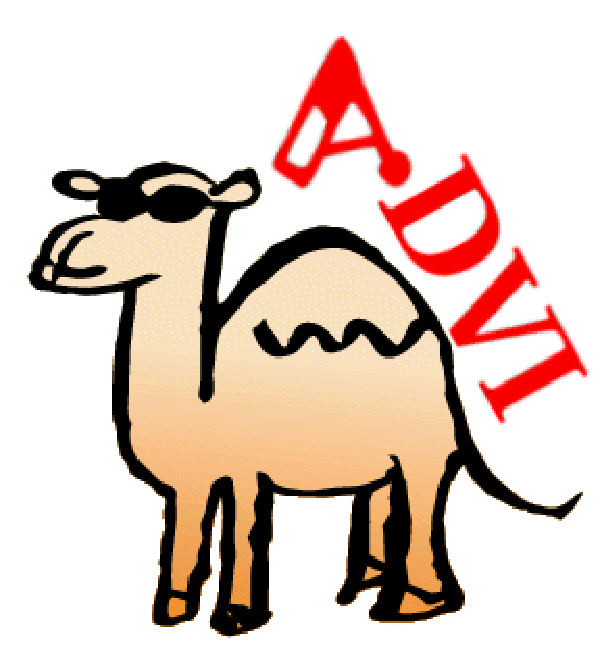
\includegraphics[width=0.5\textwidth]{../tex/advilogo.eps}\\
{\Large \bf That's all, folks!!}
\end{center}
\vfill

{\large {\bf In 10 seconds, I will quit automatically!}}

9,~\adviwait[1]
8,~\adviwait[1]
7,~\adviwait[1]
6,~\adviwait[1]
5,~\adviwait[1]
4,~\adviwait[1]
3,~\adviwait[1]
2,~\adviwait[1]
1,~\adviwait[1]
0~\adviwait[1]
\advipushkeys{"q"}

\vfill

\end{document}
